\documentclass[10pt,a4paper]{amsart}
\usepackage[utf8]{inputenc}
\usepackage[english]{babel}
\usepackage[mathcal]{euscript}
\usepackage{mathrsfs}  
\usepackage{amsmath}
\usepackage{amsfonts}
\usepackage{mathrsfs}  
\usepackage{amssymb}
\usepackage{stmaryrd}
\usepackage{graphicx}
\usepackage{mathtools}
\usepackage{pgfplots}
\usepackage{xfrac}
\usepackage{listings}
\usepackage{xcolor}
\usepackage{lstlinebgrd}
\usepackage{ebproof}
\usepackage{graphicx,float}
\usepackage[colorlinks=true, linkcolor=cyan, urlcolor=cyan, citecolor=cyan]{hyperref}
\usepackage[shortlabels]{enumitem}
\usepackage[textsize=tiny,textwidth=45]{todonotes}

\newcommand{\klcomp}{\star}
\newcommand{\parI}{\mathop{\bowtie}}
\newcommand{\seqI}{\mathop{\triangleright}}
\DeclareMathOperator{\demon}{\square}
\DeclareMathOperator{\angel}{\Diamond}
\makeatletter
\DeclareRobustCommand{\iscircle}{\mathord{\mathpalette\is@circle\relax}}
\newcommand\is@circle[2]{%
  \begingroup
  \sbox\z@{\raisebox{\depth}{$\m@th#1\bigcirc$}}%
  \sbox\tw@{$#1\square$}%
  \resizebox{!}{\ht\tw@}{\usebox{\z@}}%
  \endgroup
}
\makeatother
\DeclareMathOperator{\statt}{\iscircle_\prog{p}}
\newcommand{\schfont}[1]{\mathcal{#1}}
\newcommand{\sch}{\schfont{S}}
\newcommand{\conv}[1]{\mathrm{conv}\, {#1}}
%%%%%%%%%%%%% Macros
\newcommand{\renato}[1]{\textcolor{teal}{RN Note: #1}}
\newcommand{\codiag}{\triangledown}
%%%% Categories
\newcommand{\catfont}[1]{\mathsf{#1}}
\newcommand{\cop}{\catfont{op}}
\newcommand{\Law}{\catfont{Law}}
\newcommand{\catV}{\catfont{V}}
\newcommand{\catX}{\catfont{X}}
\newcommand{\catC}{\catfont{C}}
\newcommand{\catCat}{\catfont{C}}
\newcommand{\catCop}{\catfont{C^{op}}}
\newcommand{\catD}{\catfont{D}}
\newcommand{\catE}{\catfont{E}}
\newcommand{\catA}{\catfont{A}}
\newcommand{\catB}{\catfont{B}}
\newcommand{\catP}{\catfont{P}}
\newcommand{\catMet}{\catfont{Met}}
\newcommand{\catCPTP}{\catfont{CPTP}}
\newcommand{\catCPS}{\catfont{CPS}}
\newcommand{\catCP}{\catfont{CP}}
\newcommand{\catQ}{\catfont{Q}}
\newcommand{\catSet}{\catfont{Set}}
\newcommand{\catFinSet}{\catfont{FinSet}}
\newcommand{\catPO}{\catfont{PO}}
\newcommand{\catCompFunc}{\catfont{CompFunc}}
\newcommand{\catBan}{\catfont{Ban}}
\newcommand{\catVect}{\catfont{CVect}}
\newcommand{\WstarCPSU}{\catfont{Wstar_{CPSU}}}
\newcommand{\WstarCPSUop}{\left(\catfont{Wstar_{CPSU}}\right)^{\catfont{op}}}
\newcommand{\catI}{\catfont{I}}
\newcommand{\Set}{\catfont{Set}}
\newcommand{\Top}{\catfont{Top}}
\newcommand{\Pos}{\catfont{Pos}}
\newcommand{\Inj}{\catfont{Inj}}
\newcommand{\Det}{\catfont{RMhat}}
\newcommand{\CoAlg}[1]{\catfont{CoAlg}\left (#1 \right )}
\newcommand{\Mon}{\catfont{Mon}}
\newcommand{\Mnd}{\catfont{Mnd}(\catC)}
\newcommand{\SMnd}{\catfont{Mnd}(\Set)}
\newcommand{\CLat}{\catfont{CLat}}
\newcommand{\SLat}{\catfont{SLat}}
\newcommand{\Stone}{\catfont{Stone}}
\newcommand{\Spectral}{\catfont{Spectral}}
\newcommand{\CompHaus}{\catfont{CompHaus}}
\newcommand{\Subs}[2]{\catfont{Sub}_{}}
\newcommand{\Cone}{\catfont{Cone}}
\newcommand{\LCone}{\catfont{LCone}}
\newcommand{\StComp}{\catfont{StablyComp}}
\newcommand{\PosC}{\catfont{PosComp}}
\newcommand{\Haus}{\catfont{Haus}}
\newcommand{\Meas}{\catfont{Meas}}
\newcommand{\Coh}{\catfont{CohDom}}
\newcommand{\Ord}{\catfont{Ord}}
\newcommand{\Dcpo}{\catfont{DCPO}}
\newcommand{\Dom}{\catfont{Dom}}
\newcommand{\EndoC}{[\catC,\catC]}
\newcommand{\Dcpop}{\catfont{DCPO}^\catfont{p}}
%% General functors
\newcommand{\funfont}[1]{#1}
\newcommand{\funF}{\funfont{F}}
\newcommand{\funU}{\funfont{U}}
\newcommand{\funG}{\funfont{G}}
\newcommand{\funT}{\funfont{T}}
\newcommand{\funI}{\funfont{I}}
%% Particular kinds of functors
\newcommand{\sfunfont}[1]{\mathrm{#1}}
\newcommand{\Pow}{\sfunfont{P}}
\newcommand{\PP}{\sfunfont{V}}
\newcommand{\Dist}{\sfunfont{V}_{=1,\omega}}
\newcommand{\PDist}{\sfunfont{V}_{\leq 1,\omega}}
\newcommand{\Maybe}{\sfunfont{M}}
\newcommand{\List}{\sfunfont{L}}
\newcommand{\UForg}{\sfunfont{U}}
\newcommand{\Forg}[1]{\sfunfont{U}_{#1}}
\newcommand{\Id}{\sfunfont{Id}}
\newcommand{\Vie}{\sfunfont{V}}
\newcommand{\Disc}{\funfont{D}}
\newcommand{\Weight}{\sfunfont{W}}
\newcommand{\homf}{\sfunfont{hom}}
\newcommand{\Yoneda}{\sfunfont{Y}}
%% Diagram functors
\newcommand{\Diag}{\mathscr{D}}
\newcommand{\KDiag}{\mathscr{K}}
\newcommand{\LDiag}{\mathscr{L}}
%% Monads
\newcommand{\monadfont}[1]{\mathbb{#1}}
\newcommand{\monadT}{\monadfont{T}}
\newcommand{\monadS}{\monadfont{S}}
\newcommand{\monadU}{\monadfont{U}}
\newcommand{\monadH}{\monadfont{H}}
\newcommand{\str}{\mathrm{str}}
%% Adjunctions
\newcommand\adjunct[2]{\xymatrix@=8ex{\ar@{}[r]|{\top}\ar@<1mm>@/^2mm/[r]^{{#2}}
& \ar@<1mm>@/^2mm/[l]^{{#1}}}}
\newcommand\adjunctop[2]{\xymatrix@=8ex{\ar@{}[r]|{\bot}\ar@<1mm>@/^2mm/[r]^{{#2}}
& \ar@<1mm>@/^2mm/[l]^{{#1}}}}
%% Retractions
\newcommand\retract[2]{\xymatrix@=8ex{\ar@{}[r]|{}\ar@<1mm>@/^2mm/@{^{(}->}[r]^{{#2}}
& \ar@<1mm>@/^2mm/@{->>}[l]^{{#1}}}}
%% Limits
\newcommand{\pv}[2]{\langle #1, #2 \rangle}
\newcommand{\limt}{\mathrm{lim}}
\newcommand{\pullbackcorner}[1][dr]{\save*!/#1+1.2pc/#1:(1,-1)@^{|-}\restore}
\newcommand{\pushoutcorner}[1][dr]{\save*!/#1-1.2pc/#1:(-1,1)@^{|-}\restore}
%% Colimits
\newcommand{\colim}{\mathrm{colim}}
\newcommand{\inl}{\mathrm{inl}}
\newcommand{\inr}{\mathrm{inr}}
%% Distributive categories
\newcommand{\distr}{\mathrm{dist}}
\newcommand{\undistr}{\mathrm{undist}}
%% Closedness
\newcommand{\curry}[1]{\mathrm{curry}{#1}}
\newcommand{\app}{\mathrm{app}}
%% Misc. operations
\newcommand{\const}[1]{\underline{#1}}
\newcommand{\comp}{\cdot}
\newcommand{\id}{\mathrm{id}}
\newcommand{\sw}{\mathrm{sw}}
\newcommand{\spt}{\mathrm{sp}}
\newcommand{\sh}{\mathrm{sh}}
\newcommand{\jn}{\mathrm{jn}}
\newcommand{\dist}{\mathrm{dist}}
\newcommand{\unfold}{\mathrm{unfold}}
\newcommand{\fold}{\mathrm{fold}}
%% Factorisations
\newcommand{\EClass}{E}
\newcommand{\MClass}{M}
\newcommand{\MConeClass}{\mathcal{M}}
%%%%%%%%%%%%%%%% End of Categorical Stuff

%%%% Misc
%% Operations
\newcommand{\blank}{\, - \,}
\newcommand{\sem}[1]{\left \llbracket #1 \right \rrbracket}
\newcommand{\asem}[1]{ \llparenthesis #1 \rrparenthesis}
\newcommand{\closure}[1]{\overline{#1}}
\DeclareMathOperator{\img}{\mathrm{im}}
\DeclareMathOperator{\dom}{\mathrm{dom}}
\DeclareMathOperator{\codom}{\mathrm{codom}}
%% Sets of numbers
\newcommand{\Nats}{\mathbb{N}}
\newcommand{\Reals}{\mathbb{R}}
\newcommand{\Rats}{\mathbb{Q}}
\newcommand{\Rz}{\Reals_{\geq 0}}
\newcommand{\Complex}{\mathbb{C}}
%% Writing
\newcommand{\cf}{\emph{cf.}}
\newcommand{\ie}{\emph{i.e.}}
\newcommand{\eg}{\emph{e.g.}}
\newcommand{\df}[1]{\emph{\textbf{#1}}}
%%%%%%%%%%%%%%%% End of Misc

%%%% Programming Stuff
%% Types
\newcommand{\typefont}[1]{\mathbb{#1}}
\newcommand{\typeOne}{1}
\newcommand{\typeTwo}{2}
\newcommand{\typeA}{\typefont{A}}
\newcommand{\typeB}{\typefont{B}}
\newcommand{\typeC}{\typefont{C}}
\newcommand{\typeV}{\typefont{V}}
\newcommand{\typeD}{\typefont{D}}
\newcommand{\typeE}{\typefont{E}}
\newcommand{\typeF}{\typefont{F}}
\newcommand{\typeI}{\typefont{I}}
%% RuleName
\newcommand{\rulename}[1]{(\mathrm{#1})}
%% Sequents
\newcommand{\jud}{\vdash}
\newcommand{\vljud}{\triangleright}
\newcommand{\cojud}{\vdash_{\co}}
\newcommand{\vl}{\mathtt{v}}
\newcommand{\co}{\mathtt{c}}
% Program font
\newcommand{\prog}[1]{\ensuremath{\tt #1}}
\newcommand{\blue}[1]{\textcolor{blue}{#1}}
\newcommand{\pseq}[3]{#1 \leftarrow #2; #3}
\newcommand{\ppm}[4]{(#1,#2) \leftarrow #3; #4}
\newcommand{\pinl}[1]{\prog{inl}(#1)}
\newcommand{\pinr}[1]{\prog{inr}(#1)}
\newcommand{\pcase}[5]{\prog{ case } #1 \prog{ \hspace{2pt} of \hspace{2pt} } \pinl{#2} \Rightarrow #3 ; \pinr{#4} \Rightarrow #5}
%% Sets of terms
\newcommand{\ValuesBP}[2]{\mathsf{Values}(#1, #2)}
\newcommand{\TermsBP}[2]{\mathsf{Terms}(#1, #2)}
\newcommand{\closValP}[1]{\ValuesBP{\emptyset}{#1}}
\newcommand{\closTermP}[1]{\TermsBP{\emptyset}{#1}}
\newcommand{\closVal}{\closValP{\typeA}}
\newcommand{\closTerm}{\closTermP{\typeA}}
%% Contextual equivalence
\newcommand{\ctxeq}{\equiv_{\prog{ctx}}}

%%%% End of Programming Stuff
\newcommand{\Shuff}{\mathrm{Sf}}

%%%% Domain theory
\newcommand{\upclos}{\mathord{\uparrow}}
\newcommand{\dwclos}{\mathord{\downarrow}}

%%%% Quantum stuff
\newcommand{\Hilb}{\catfont{Hilb}}
\newcommand{\tr}{\text{Tr}}

%%%% Norms
\newcommand{\euclideannorm}[1]{\left\lVert #1  \right\rVert_{2}}
\newcommand{\spectralnorm}[1]{\left\lVert #1  \right\rVert_{\infty}}
\newcommand{\tracenorm}[1]{\left\lVert #1  \right\rVert_{1}}
\newcommand{\diamondnorm}[1]{\left\lVert #1  \right\rVert_{\diamondsuit}}
\newcommand{\lonenorm}[1]{\left\lVert #1  \right\rVert_{ L^{1} }}
\newcommand{\gentracenorm}[1]{\left\lVert #1  \right\rVert_{ L^\infty }}
\newcommand{\gendiamondnorm}[1]{\left\lVert #1  \right\rVert_{ \diamondsuit \text{ gen}}}
\newcommand{\opnorm}[1]{\left\lVert #1  \right\rVert_{\text{op}}}
\newcommand{\norm}[1]{\left\lVert #1  \right\rVert}
\newcommand{\cbnorm}[1]{\left\lVert #1  \right\rVert_{\text{cb}}}
\newcommand{\projnorm}[1]{\left\lVert #1  \right\rVert_{\pi}}

%%%% Tensor
\newcommand{\projtensor}{\widehat{\otimes}_\pi}

\usepackage[left=2cm,right=2cm,top=2cm,bottom=2cm]{geometry}
\usepackage{tcolorbox}
\usepackage{braket}
\usepackage{quantikz}
\usepackage{tikz-cd}
\linespread{1.10}
\author{\dots}
\title{Notes}
\pgfplotsset{compat=1.18}

\lstset{
language=C,
showstringspaces=false,
keywordstyle=\color{blue},
basicstyle=\fontsize{10}{13}\ttfamily,
emph={exit,blue,unif,then,wait},emphstyle=\color{blue},
breaklines=true,
escapeinside={*@}{*@}
}


\usepackage{proof}
\usepackage{amsthm}
\usepackage[all]{xy}
%for definition
\theoremstyle{definition}
\newtheorem{definition}{Definition}[section]

%for examples
\theoremstyle{definition}
\newtheorem{example}[definition]{Example}

%lemmas
\theoremstyle{definition}
\newtheorem{lemma}[definition]{Lemma}

%proposition
\theoremstyle{definition}
\newtheorem{proposition}[definition]{Proposition}
%corollary
\theoremstyle{definition}
\newtheorem{corollary}[definition]{Corollary}

%theorem
\theoremstyle{definition}
\newtheorem{theorem}[definition]{Theorem}

% Renato's macros
\newcommand{\until}{\> \textcolor{blue}{\prog{for}} \>}
\newcommand{\then}{\textcolor{blue}{then}}
\newcommand{\progife}[3]{{ \blue{\prog{if}} \> #1 \> \blue{\prog{then}} \> 
{\prog #2} \> \blue{\prog{else}} \> {\prog #3}}}
\newcommand{\progwhile}[2]{{\blue{\prog{while}} \>  #1 \> \blue{\prog{do}} \> \{ \> {#2}  \> \}}}
\newcommand{\scomp}{\, \blue{;} \,}
\newcommand{\prem}[1]{(\text{if\/ }#1)}
\newcommand{\nline}{\vspace{-5mm}}
\newcommand{\ssto}[1][]{~\to^{#1}~}
\newcommand{\bsto}{~\Downarrow~}
\newcommand{\stp}{\mathit{stop}}
\newcommand{\skp}{\mathit{skip}}
\newcommand{\err}{\mathit{err}}
\providecommand{\comma}{,\operatorname{}\linebreak[1]}		% possibly line-beaking comma
\newcommand{\sep}{\kern1pt\comma\kern-1pt}
\newcommand{\lrule}[3]{\textbf{#1}\quad\frac{#2}{#3}}
\newcommand{\ptt}{{\prog tt}}
\newcommand{\pff}{{\prog ff}}
\newcommand{\unif}{{\prog \blue{unif}}}
\newcommand{\meas}[1]{\mathcal{M}(#1)}
\newcommand{\pmap}{ \xrightharpoonup{\hspace{0.1cm}} }

\begin{document}
\title{Xelatex is bloated}
\maketitle
\section{Probabilistic computation} \label{subsec:syntax_pc}

We now briefly illustrate the case of probabilistic computation, using as basic
examples two main topics in probability theory~\cite{dudley18} -- probabilistic
predicates and random walks on the real line.  Our illustration will be
grounded on a standard probabilistic model, namely the category $\Ban$ of
Banach spaces and linear contractions~\cite{dahlqvist19}. As discussed
in~\cite{dahlqvist2023syntactic} this category has a $\Met$-enriched
monoidal-closed structure and it is well-known that it has binary coproducts
given by the direct sum equipped with the $\ell_1$ norm. Thus in order to fit
$\Ban$ in our framework we only need to show that its binary coproduct
structure is $\Met$-enriched as well. We prove this next. 

Let us start with some preliminaries. The $\Met$-enriched structure of $\Ban$
is induced by the \emph{operator norm}. Specifically given a linear map 
$T : V \to W$ between Banach spaces we have,
\[
        \norm{T} = \sup \{ \norm{T(v)} \mid v \in V, \norm{v} = 1 \}
\]
Linear contractions will be precisely those linear maps $T$ such that $\norm{T}
\leq 1$, and the distance between two contractions $T$ and $S$ is set as
$\norm{ T - S}$. Given $T : V \to W$ and $S : U \to W$ their co-pairing $[T,S]
: V \oplus U \to W$ is defined by $[T,S](v,u) = T(v) + S(u)$. The fact that the
operator $[T,S]$ is contractive follows from the inequation $\norm{[T,S]} \leq
\max \{ \norm{T}, \norm{S} \}$ -- which is straightforward to prove when
one notices that every unitary vector $(v,u) \in V \oplus U$ can be rewritten
as,
\[
        \left (\norm{v} \frac{1}{\norm{v}} v, \norm{u} \frac{1}{\norm{u}} u \right )
        \hspace{1cm}
        \norm{v} + \norm{u} = 1
\]
The fact that the coproduct structure of $\Ban$ is $\Met$-enriched then follows
rather directly,
\begin{align*}
        d([T,S] , [T',S']) 
        & = 
        \norm{ [T,S] - [T',S'] }
        \\
        & = 
        \norm{ [T - T', S - S'] }
        \\
        & \leq
        \max \{ \norm{T - T'}, \norm{S - S'} \}
        \\
        & =
        \max \{ d(T,T'), d(S,S') \}
\end{align*}
Next, we will involve the notion of a measure (see \eg\ \cite[Chapter
10]{aliprantis06} or \cite[Chapter 2]{panangaden09}).

\begin{definition} For a measurable space $(X,\Sigma_X)$ a measure is a
        function $\mu : \Sigma_X \to \Reals$ such that $\mu(\emptyset) = 0$ and
        moreover it is $\sigma$-additive, \ie\ 
        \[
        \mu \left (\bigcup_{i =1}^{\infty} U_i \right ) = \sum_{i = 1}^{\infty}
        \mu(U_i) 
        \] 
where $(U_i)_{i \in \omega}$ is any family of pairwise disjoint measurable
sets.  A measure $\mu$ is called positive if $\mu(U) \geq 0$ for all measurable
sets $U$.  
\end{definition}

For a measurable space $X$ the set of measures $\Measu(X)$ forms a vector space
via pointwise extension. It also forms a Banach space when equipped with the
total variation norm,
\[
        \lVert \mu \rVert = 
        \sup \left \{ \sum_{i = 1}^n \, \lVert \mu(U_i) \rVert \mid
             \{ U_1, \dots, U_n \} \text{ is a measurable partition }
        \right \}
\]
An extremely useful fact is that $\norm{\mu} = \mu^{+}(X) + \mu^{-}(X)$ where
$\mu^{+}$ and $\mu^{-}$ are the positive and negative parts of $\mu$
respectively (see details in~\cite[Section 8.2. and Section
10.10]{aliprantis06}).

We proceed by presenting a simple a metric $\lambda$-theory on which to reason
about predicates and random walks, as previously discussed. Our (only) ground
type will be $\mathtt{real}$ to represent measures over real numbers, \ie\ we
set $\sem{\mathtt{real}} = \Measu(\Reals)$.  Concerning operations we take a
pre-determined set of predicates $p : \mathtt{real} \to \typeI \oplus \typeI$,
whose interpretation takes the form $\sem{p}(\mu) = (\mu(U),
\mu(\overline{U}))$ for some measurable subset of $U \subseteq \Reals$. In
other words $U \subseteq \Reals$ corresponds to the subspace in which the
predicate is supposed to hold. We also take a pre-determined set of actions $a
: \typeI \to (\typeA \multimap \typeA)$ and a pre-determined set of measures $m
: \typeI \to \mathtt{real}$, whose interpretation takes no particular form.
Now, given a measure $m$ and actions $a,b$ consider the following
'abstract' Bernoulli trial,
\[
        p : \mathtt{real} \multimap \typeI \oplus \typeI
        \vljud \underbrace{ \text{case } p(m) \text{ of } \inl(x) \Rightarrow a(x) ; 
        \inr(y) \Rightarrow b(y)}_{\mathtt{bern}(p)} : \typeA \multimap \typeA
\]
Note that if $p_1(x) =_\epsilon p_2(x)$ then  $\mathtt{bern}(\lambda x. p_1(x))
=_\epsilon \mathtt{bern}(\lambda x. \, p_2(x))$ holds, as per our equational
system. Such is useful to approximate Bernoulli trials that are hard to compute
as the following example illustrates.
\begin{example}[Predicates as limits of Cauchy sequences]
        Consider the predicate,
        \[
                x : \mathtt{real} \vljud
                p_{\frac{1}{2}\sqrt{2}}(x) : \typeI \oplus \typeI
        \]
        that returns true if $x < \frac{1}{2}\sqrt{2}$ and false otherwise.
        Given the irrationality of $\frac{1}{2}\sqrt{2}$ it is natural to
        consider successive approximations $p_{q_n}(x) :  \typeI \oplus \typeI$
        $(n \in \Nats)$ of this predicate in which the condition $x <
        \frac{\sqrt{2}}{2}$ is replaced by $x < q_n$ for $q_n$ a rational
        number. We show next how our framework makes this idea precise. Take
        the sequence of rational numbers $(q_n)_{n \in \Nats}$ defined by,
        \[
                \begin{cases}
                        q_0 & = 1
                        \\
                        q_{n + 1} & = \frac{1}{2} (q_n + \frac{2}{q_n})
                \end{cases}
        \]
        which corresponds to Heron's method for approximating $\sqrt{2}$ (\ie\
        $\lim_{n \to \infty} q_n = \sqrt{2}$). We then postulate as axioms in
        our deductive system that $(p_{\frac{1}{2} q_n}(x))_{n \in \Nats}$ is a
        Cauchy sequence and furthermore that it converges to $p_{\frac{1}{2}
        \sqrt{2}}(x)$.  Such is asserted explicitly by setting,
        \begin{equation}
                \label{eq:sound}
                \begin{cases}
                \forall \epsilon > 0. \, \exists m \in \Nats.
                \, \forall n \geq m. \, p_{\frac{1}{2}q_n}(x) =_\epsilon p_{\frac{1}{2}q_{n+1}} (x)
                & \text{(Cauchy sequence)}
                \\
                \forall \epsilon > 0. \, \exists m \in \Nats.
                \, \forall n \geq m. \, p_{\frac{1}{2}q_n}(x) 
                =_\epsilon p_{\frac{1}{2} \sqrt{2}} (x)
                & \text{(Convergence)}
                \end{cases}
        \end{equation}
        for appropriate choices of $m$ (which in our context is irrelevant to
        detail). Then note that according to our deductive system we have that
        $\mathtt{bern}(\lambda x. \, p_{\frac{1}{2} q_n}(x))_{n \in \Nats}$ is
        a Cauchy sequence that furthermore converges to $\mathtt{bern}(\lambda
        x. \, p_{\frac{1}{2} \sqrt{2}}(x))$. Then next step is to prove
        that our axiomatics is sound.
        \begin{align*}
                \sem{p_{\frac{1}{2} \sqrt{2}}(x)}(\mu)
                & = \left (\mu \left (-\infty, \frac{1}{2} \sqrt{2} \right ), 
                \mu(X) - \mu \left (-\infty, \frac{1}{2}\sqrt{2} \right ) \right )
                &
                \\
                & = \left (\mu \left (\bigcup_{n \in \Nats} 
                        \left (-\infty, \frac{1}{2} q_n \right )\right ), 
                \mu(X) - \mu \left (-\infty, \frac{1}{2}\sqrt{2} \right ) \right )
                & 
                \left \{(\frac{1}{2}q_n)_{n \in \Nats} 
                \nearrow \frac{1}{2}\sqrt{2} \right \}
                \\
                & = \left (\sup_{n \in \Nats} \mu \left ( 
                        \left (-\infty, \frac{1}{2} q_n \right )\right ), 
                \mu(X) - \mu \left (-\infty, \frac{1}{2}\sqrt{2} \right ) \right )
                & 
                \left \{ \text{Measure properties} \right \}
                \\
                & = \left (\lim_{n \to \infty} \mu \left ( 
                        \left (-\infty, \frac{1}{2} q_n \right )\right ), 
                \mu(X) - \mu \left (-\infty, \frac{1}{2}\sqrt{2} \right ) \right )
                & 
                \left \{ \text{Limits coincide with sup. of inc. seq.} \right \}                         \\
                & = \left (\lim_{n \to \infty} \mu \left ( 
                        \left (-\infty, \frac{1}{2} q_n \right )\right ), 
                \lim_{n \to \infty}
                \mu \overline{\left (-\infty, \frac{1}{2}q_n \right )} \right )
                & 
                \left \{ \text{Measure properties} \right \}
                \\
                & = \lim_{n \to \infty} \left (\mu \left ( 
                        \left (-\infty, \frac{1}{2} q_n \right )\right ), 
                \mu \overline{\left (-\infty, \frac{1}{2}q_n \right )} \right )
                & 
                \\
                & = \lim_{n \to \infty}
                \sem{p_{\frac{1}{2}q_n}(x)}(\mu)
                &
        \end{align*}
\end{example}

\begin{example}[From predicates approximation to random walk approximation] 
        Let us now capitalise on the previous example to reason about
        approximations of random walks. First consider the term,
        \[
                (-) \vljud \underbrace{\lambda x_1. \, \dots \, x_k. \, y. \,
                x_1 (\dots (x_k(y)) \dots)}_{\mathtt{sequence_k}}
        \]
        which sequences $k$ terms given as input. Then take the $\lambda$-term
        $\mathtt{sequence_k} \> \mathtt{bern}(\lambda x. \, p(x)) \dots \,
        \mathtt{bern}(\lambda x. \, p(x)) : \typeA \to \typeA$ which
        intuitively represents an abstract random walk of $k$-steps. In order
        to keep our notation simple we will abbreviate this last $\lambda$-term to
        $\mathtt{rwalk}(\lambda x. \, p(x))$.  It follows from our system that
        if $p_1(x) =_\epsilon p_2(x)$ then,
        \[
                \mathtt{rwalk}(\lambda x. p_1(x)) =_{n \cdot \epsilon}
                \mathtt{rwalk}(\lambda x. p_2(x)) 
        \]
        In particular from the previous example we can deduce that
        $\mathtt{rwalk}\left (\lambda x. \, p_{\frac{1}{2} q_n} (x) \right )$
        is a Cauchy sequence that converges to $\mathtt{rwalk}\left (\lambda x.
        \, p_{\frac{1}{2} \sqrt{2}} (x) \right )$.

        As a final illustration we suppose now that the actions $a,b : \typeA
        \to \typeA$ involved in $\mathtt{bern}(\lambda x. \, p(x))$ are
        concrete jumps on the real line. To this effect,
        we set,
        \[
                        \sem{a}(1)(\mu) = +_\ast(\mu \otimes \mathtt{unif}(0,v))
                        \hspace{2cm}
                        \sem{b}(1)(\mu) = +_\ast(\mu \otimes \mathtt{unif}(-v,0))
        \]
        where $v \in \Rz$, $+_\ast$ is the pushforward measure of $+ : \Reals
        \times \Reals \to \Reals$, $\mathtt{unif}(0,v)$ is the uniform measure
        on the interval $[0,v]$ and analogously for $\mathtt{unif}(-v,0)$. Thus
        operationally $a$ corresponds to a jump to the right with magnitude not
        exceeding $v$ and analogously for $b$. Suppose then we have another
        action $c : \typeI \to (\mathtt{real} \multimap \mathtt{real})$ whose
        interpretation is that of $a$ except for the fact that
        $\mathtt{unif}(0,v)$ is replaced by $\mathtt{unif}(0,v+\delta)$. What
        will be the effect on the random walk when replacing $a$ by $c$? The
        idea is first to postulate a suitable metric axiom that relates $a$
        with $c$.
\end{example}




  \begin{example}[Random walk]

    $\mathbf{Ban}$ provides a model of the metric $\lambda$-theory presented in \ref{ex:random_walk_prob}  via the following interpretation: $\sem{\emph{real}} = \mathcal{M}\mathbb{R}$, the Banach space of finite Borel measures on $\mathbb{R}$ equipped with the total  variation norm.

    For a finite measure $\nu$, the total variation norm is defined as
    \begin{align*}
      \norm{\nu} = \sup \left\{ \sum_{i=1}^n |\nu(A_i)| \mid A_i \in \mathcal{B}(\mathbb{R}), A_i \cap A_j = \emptyset, i \neq j, n \in \mathbb{N} \right\}
    \end{align*}



    The following alternative definition is useful to compute the total variation norm between measures.

  \begin{definition} \cite{tsybakov2008}
    Let  let $P$ and $Q$ be two probability measures on $\mathcal{M}\mathbb{R}$. Define
    $$
      \nu = P + Q, \quad p = \frac{dP}{d\nu}, \quad q = \frac{dQ}{d\nu},
    $$
    where $\frac{dP}{d\nu}$ denotes the  the Radon–Nikodym derivative of the measure $P$ with respect to the measure $\nu$. It holds that:
    \begin{align*}
      \norm{P-Q} = \sup \left\{ 2 \cdot \left\vert \int_{A} (p - q) \, d\nu \mid A \in  \mathcal{B}(\mathbb{R}) \right\vert \right\}
    \end{align*}
  \end{definition}
  
    Returning to the interpretation of our $\lambda$-theory, 
    we have $I = \mathbb{R} \ni 1$, 
    for every $r \in \mathbb{Q}$ we define $\sem{\emph{delta}_r}:\mathbb{R} \to \mathcal{M}\mathbb{R},\ x \mapsto x\delta_r$, where $\delta_r$ is the Dirac delta over $r$. 
    Similarly for every $r,s \in \mathbb{Q}$ we have $\sem{\emph{u}_{r,s}}:\mathbb{R} \to \mathcal{M}\mathbb{R},\ 1 \mapsto U(r,s) $, where $U_{r,s}$ denotes the continous uniform distibution, with $r$ and $s$ as the minimum and maximum values, respectively. 
    Next,  for every $p_1,\ldots,p_n \in [0,1]$, we have $\sem{\emph{delta}_{p_1,\ldots,p_n}}:\mathbb{R} \to \mathcal{M}\mathbb{R},\ 1 \mapsto \sum_{i=1}^n p_i\cdot \delta_{x_i}$, where $x_i \in \mathbb{Q}$
    Moreover  for every $p \in [0,1]$ we define $\sem{\emph{CoinToss}_p}:\mathbb{R} \to \mathbb{R} \oplus \mathbb{R},\ 1 \mapsto (p, 1-p)$. 
    Finally for every $\mu \in \mathcal{M}\mathbb{R}$ and for $\nu  \in \mathcal{M}\mathbb{R}$ we define $\sem{\emph{JumpL}_\mu} (\nu) = jl_{*}(\mu,\nu) $, the pushforward of the product measure $\mu \otimes \nu$ (seen as an element of $\mathcal{M}(\mathbb{R} \times \mathbb{R})$) under the Markov kernel $jl: \mathbb{R}^2 \to \mathcal{M}\mathbb{R},\ (u,v) \mapsto \delta_{v-u}$.  We define an analogous interpretation for the sampling function $\sem{\emph{JumpR}_\mu}$ considering the Markov kernel $jr: \mathbb{R}^2 \to \mathcal{M}\mathbb{R},\ (u,v) \mapsto \delta_{v+u}$.

    Let us consider that in operations $\emph{CoinToss}_p$, $\emph{JumpL}_{\mu_1}$, $\emph{JumpR}_{\mu_1}$, the parameters $p, \mu_1$ and $\mu_2$ are afected by errors and in actuality we have operations $\emph{CoinToss}_{p'}$, $\emph{JumpL}_{\mu_{1'}}$, $\emph{JumpR}_{\mu_{2'}}$. 
    If we have axioms 
    $\emph{CoinToss}_p (*) =_{\epsilon_1}\emph{CoinToss}_{p'}(*)$, 
    $\emph{JumpL}_{\mu_1} =_{\epsilon_2}\emph{JumpL}_{\mu_{1'}}$, and $\emph{JumpR}_{\mu_2} =_{\epsilon_3}\emph{JumpR}_{\mu_{2'}}$, using our metric deductive system it follows that 
    $$\textbf{step} =_{\epsilon_1 + \max\{\epsilon_2, \epsilon_3\}} \textbf{step}^{\epsilon_1, \epsilon_2, \epsilon_3},$$
    where $\textbf{step}^{\epsilon_1, \epsilon_2, \epsilon_3}$ corresponds to the $\lambda$-term resulting from the substitution of operations $\emph{CoinToss}_p$, $\emph{JumpL}_{\mu_1}$ and $\emph{JumpL}_{\mu_2}$ by their erroneous versions. 
    Finally, designating $\textbf{rwalk-n}^{\epsilon_1, \epsilon_2, \epsilon_3}$ as the judgement that results from replacing $\textbf{step}$ by $\textbf{step}^{\epsilon_1, \epsilon_2, \epsilon_3}$, we can infer,
    $$\textbf{rwalk-n} =_{n \cdot (\epsilon_1 + \max\{\epsilon_2, \epsilon_3\})} \textbf{rwalk-n}^{\epsilon_1, \epsilon_2, \epsilon_3},$$

      


    Let us now verify that we can in fact build the axioms previouly mentioned based on our model.


   

  Considering the absolute value as the norm on real numbers, it follows that
  \begin{align*}
    \norm {\sem{\emph{CoinToss}_p(*)} - \sem{\emph{CoinToss}_q(*)}} & = \norm {(p,1-p) - (q, 1-q)} \\
    & =\norm {(p-q,q-p)}  = 2|p-q|
  \end{align*}

  As a result we can postulate the following metrix axiom:
  $$ \emph{CoinToss}_p(*) =_{2|p-q|} \emph{CoinToss}_q(*)$$


  Given a finite set of natural numbers \(N = \{1, \ldots, n\}\), let \(\mu \in \mathcal{M}(N)\) be a probability measure. Then \(\mu\) can be expressed as
  \[
  \mu = \sum_{i=1}^{n} p_i \delta_i,
  \]
  where each \(p_i\) is the probability assigned to \(i \in N\), and \(\delta_i\) denotes the Dirac measure at \(i\).

    Consequently, we have that 
    $$ \norm{\mu} =  \norm{\sum_{i=1}^{n} p_i \delta_i} = \sum_{i=1}^{n} p_i$$

    Note that there is an isomorphism $ \mathbb{R} \times \mathbb{R}  \cong \mathcal{M}(1+1)$, given by $\phi: \mathcal{M}(1+1) \to \mathbb{R} \to \mathbb{R}  ,\ p_x \delta_x + p_y \delta_y  \mapsto (p_x, p_y)$. 

  


    


    % considerando as props do tensor
    
    %RACIOCINIO: 
    % 1ª op: \nu -> \nu \otimes 1
    %no final de aplicarmos \id otimes f temos \nu \otimes \mu
    % se houver um erro com f teremos \mu \otimes \mu'
    % se sabemos a distancia entre mu e mu' estamos safos porque a seguir estamos a aplicar ops predefinidas e aí somam-se os erros dos argumentos

     \todo[inline,size=\normalsize]{Problema notação: tensor e product measure} 

    %Let $i_1: \mathcal{M}\mathbb{R}  \to \mathbb{R} \otimes \mathcal{M}\mathbb{R}$ be the isomophism defined as $i_1(\nu) = 1  \widehat{\otimes}_{\pi} \nu$. 
    %This isomorphism is clearly a short map given that $ 1  \widehat{\otimes}_{\pi} \nu = \nu$. 
    Consider the isomorphism $i_2: \mathcal{M}\mathbb{R} \,   \widehat{\otimes}_{\pi} \,   \mathcal{M}\mathbb{R} \to  \mathcal{M} \left( \mathbb{R} \times \mathbb{R} \right),$ 
    $\mu  \widehat{\otimes}_{\pi} \nu \to \mu \otimes \nu.$ 
    The product measure $\mu \otimes \nu$ is defined as $\mu  \otimes \nu (A \times B)= \mu(A)\cdot\nu(B).$
    This is the measure produced by the Carath\'{e}odory's extension theorem \cite{aliprantisBanachLattices1999}.
    Given that $\norm{\mu \otimes \nu}= |\mu (\mathbb{R})|\cdot |\nu (\mathbb{R})| = \norm{\mu} \cdot \norm{\nu}$, and $ \norm{\mu \, \widehat{\otimes}_{\pi} \, \nu} = \norm{\mu} \cdot \norm{\nu}$ (the projective norm is a cross norm) it follows that $i_2$ is a short map.



    % Isto só funcinava se nos restrigissemos a M[0,1]
    \begin{comment}
    Next, consider the following commutative diagram:

    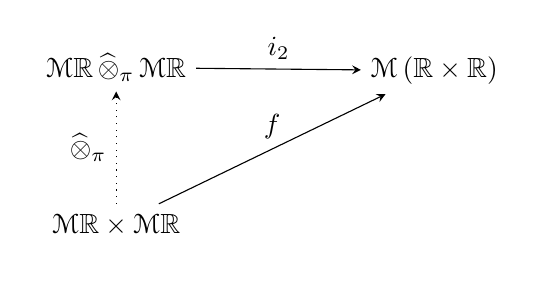
\begin{tikzpicture}
      \matrix (m) [matrix of math nodes, row sep=4em, column sep=6em, minimum width=2em]
      {
         \mathcal{M}\mathbb{R} \,   \widehat{\otimes}_{\pi} \,   \mathcal{M}\mathbb{R} &  \mathcal{M} \left( \mathbb{R} \times \mathbb{R} \right)  \\
        \mathcal{M}\mathbb{R} \times \mathcal{M}\mathbb{R}   \\
      };
      \path[dotted, -stealth]
      (m-2-1) edge node [left] {$\widehat{\otimes}_{\pi}$} (m-1-1);
      \path[-stealth]
        (m-1-1) edge node [above] {$i_2$} (m-1-2)
        (m-2-1) edge node [above] {$f$} (m-1-2)
        ;
    \end{tikzpicture}

    Where $i_2:  \mathcal{M}\mathbb{R} \,   \widehat{\otimes}_{\pi} \,   \mathcal{M}\mathbb{R} \to  \mathcal{M} \left( \mathbb{R} \times \mathbb{R} \right) $ is an isomorphism defined as $i_{2}( \mu  \widehat{\otimes}_{\pi} \nu ) = \mu \otimes \nu $ 
    and the function $f: \mathcal{M}\mathbb{R} \times \mathcal{M}\mathbb{R}  \to \mathcal{M} \left( \mathbb{R} \times \mathbb{R} \right) $ is defined as $f((\mu, \nu)) = \mu \otimes \nu $. 
    The product measure $\mu \otimes \nu$ is defined as $\mu \otimes \nu (A \times B)= \mu(A)\cdot\nu(B).$
      This is the measure produced by the Carath\'{e}odory's extension theorem \cite{aliprantisBanachLattices1999}.
       Given that $\norm{\mu \otimes \nu}= \norm{\mu} \cdot \norm{\nu}$,  and $\norm{(\mu, \nu)}= \max\{\norm{\mu}, \norm{\nu}\}$, for $\norm{\mu} \leq 1$ and $\norm{\nu} \leq 1$, it follows that $f$ is a short map.

    \end{comment}

    Since the diagram below commutes, and all the operations involved are short maps (considering $f$ as $\sem{\emph{delta}_r}$ or $\sem{\emph{u}_{r,s}}$), it follows that, if $d(\mu, \mu')=\epsilon$, then we may postulate \(\emph{JumpL}_\mu =_{\epsilon} \emph{JumpL}_{\mu'}\). A similar diagram can be constructed using \(jr_{*}\), allowing us to apply the same reasoning to the corresponding axioms.

    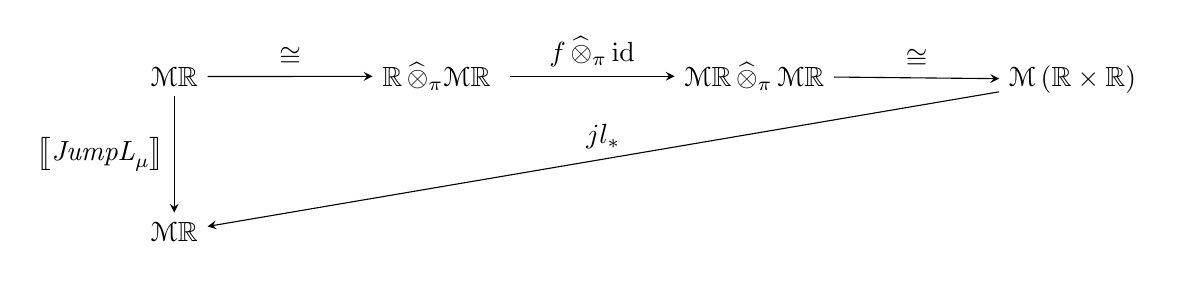
\begin{tikzpicture}
      \matrix (m) [matrix of math nodes, row sep=4em, column sep=6em, minimum width=2em]
      {
        \mathcal{M}\mathbb{R}  & \mathbb{R} \,   \widehat{\otimes}_{\pi} \mathcal{M}\mathbb{R} \,  \, & \mathcal{M}\mathbb{R} \, \widehat{\otimes}_{\pi} \,  \mathcal{M}\mathbb{R} &  \mathcal{M} \left( \mathbb{R} \times \mathbb{R} \right)  \\
        \mathcal{M}\mathbb{R}  \\
      };
      \path[-stealth]
        (m-1-1) edge node [left] {$\sem{\emph{JumpL}_\mu}$} (m-2-1)
        (m-1-1) edge node [above] {$\cong$} (m-1-2)
        (m-1-2) edge node [above] {$f\,  \widehat{\otimes}_{\pi} \,  \id $} (m-1-3)
        (m-1-3) edge node [above] {$\cong$} (m-1-4)
        (m-1-4) edge node [above] {$jl_{*}$} (m-2-1)
        ;
    \end{tikzpicture}

   We now present examples of \(\mu\) and \(\mu'\), and demonstrate how to compute the distance between them.
    First, consider $\mu=\delta_x$ and  $\mu'=\delta_y$. We calculate

    \begin{align*}
      \norm{\delta_x - \delta_y} = \sup \left\{ \sum_{i=1}^{n} |\delta_x - \delta_y (A_i)| \mid A_i \in \mathcal{B}(\mathbb{R}), A_i \cap A_j = \emptyset i,  \neq j, n \in \mathbb{N}  \right\} = 2
    \end{align*}
    Note that there are only two possibilities: either \(\delta_x\) and \(\delta_y\) belong to the same partition, or they belong to different ones. In the first case, we have
    \[
    \sum_{i=1}^{n} \left| \delta_x(A_i) - \delta_y(A_i) \right| = |1 - 1| = 0,
    \]
    while in the second case, we obtain
    \[
    \sum_{i=1}^{n} \left| \left( \delta_x(A_i) - \delta_y(A_i) \right) \right| = |1| + |-1| = 2.
    \]
    
    Next, take $\mu= \sum_{i=1}^{n} p_i \delta_{x_i}$ and  $\mu'= \sum_{i=1}^n q_i \delta_{x_i}$. We compute

    \begin{align*}
      \norm{\sum_i p_i \delta_{x_i} - \sum_i q_i \delta_{x_i}} &
      = \sup \left\{ \sum_{i=1}^{n} \left\lvert \left(\sum_i p_i \delta_{x_i} - \sum_i q_i \delta_{x_i} \right) (A_i) \right\rvert \,\Bigg| \, A_i \in \mathcal{B}(\mathbb{R}), A_i \cap A_j = \emptyset i,  \neq j, n \in \mathbb{N}  \right\} \\
      & = \sum_i |p_i-q_i|
    \end{align*}
    Here, we apply the same reasoning as in the previous example, while also using the inequality
\[
\left| \sum_{i=1}^{n} a_i \right| \leq \sum_{i=1}^{n} |a_i|, \quad \text{for all } n \in \mathbb{N}.
\]

Subsequently, let $\mu = U(a,b)$ and  $\mu'=U(c,d)$, such that the intervals $[a,b]$ and $[c,d]$ are disjoint ($[a, b] \cap [c, d] = \emptyset$). Then, the Radon-Nikodym derivatives (probability density functions) with respect to \( \nu = U(a, b) + U(c, d) \) are given by:

\[
\frac{dU(a, b)}{d\nu}(x) = u(a,b)(x) = 
\begin{cases} 
\frac{1}{b - a} & \text{if } x \in [a, b], \\ 
0 & \text{otherwise},
\end{cases}
\]
and similarly,
\[
\frac{dU(c, d)}{d\nu}(x) = u(c,d)(x) = 
\begin{cases} 
\frac{1}{d - c} & \text{if } x \in [c, d], \\ 
0 & \text{otherwise}.
\end{cases}
\]

Here, similarly to the first example, we calculate
\begin{align*}
  &\norm{U(a,b)-U(c,d)} = 2 \cdot \sup_{A \in \mathcal{B}(\mathbb{R})}  \left\{ \left\vert\int_A (u(a,b)(x)- u(c,d)(x)) \, d \nu(x) \right\vert \right\} \\
  & = 2 \cdot \sup_{A \in \mathcal{B}(\mathbb{R})}  \left\{ \left\vert\int_A (u(a,b)(x)) \, d \nu(x)  - \int_A (u(c,d)(x)) \,  d\nu(x) \right\vert \right\} = 2
\end{align*}

\begin{comment}
Here, we calculate
\begin{align*}
  \norm{U(a,b)-U(c,d)} = 2 \cdot \sup_{A \in \mathcal{B}(\mathbb{R})}  \left\{ \left\vert\int_A (u(a,b)(x)- u(c,d)(x)) \, dx \right\vert \right\} = 2 \cdot \sup_{A \in \mathcal{B}(\mathbb{R})}  \left\{ \left\vert\int_A (u(a,b)(x)- u(c,d)(x)) \, dx \right\vert \right\}
\end{align*}

In this case, we consider three scenarios: 
\begin{enumerate}
    \item The intervals are disjoint: \([a, b] \cap [c, d] = \emptyset\),
    \item One interval is fully contained in the other: for example, \([c, d] \subseteq [a, b]\) (or vice versa),
    \item The intervals intersect, but neither is fully contained in the other.
\end{enumerate}

In the first case, we have
\begin{align*}
  \int |u(a,b)(x)- u(c,d)(x)| \, dx  & = \int_a^b |u(a,b)(x)- u(c,d)(x)| \, dx + \int_c^d |u(a,b)(x)- u(c,d)(x)| \, dx \\
  & = \left\lvert \frac{b-a}{b-a}\right\rvert + \left\lvert- \frac{d-c}{d-c}\right\rvert = 2
\end{align*}

Regarding the second case, we compute
\begin{align*}
  \int |u(a,b)(x)- u(c,d)(x)| \, dx  & = \int_a^c |u(a,b)(x)- u(c,d)(x)| \, dx + \int_c^d |u(a,b)(x)- u(c,d)(x)| \, dx  \\
   & \hspace{10pt }+\int_d^b |u(a,b)(x)- u(c,d)(x)| \, dx \\
  & =  =  \frac{c-a}{b-a} + - (d-c) \left(\frac{1}{b-a} - \frac{1}{d-c}  \right)+  \frac{b-d}{b-a}
\end{align*}

At last, we calculate,
\begin{align*}
  \int |u(a,b)(x)- u(c,d)(x)| \, dx  & = \int_a^c |u(a,b)(x)- u(c,d)(x)| \, dx + \int_c^b |u(a,b)(x)- u(c,d)(x)| \, dx  \\
   & \hspace{10pt }+\int_b^d |u(a,b)(x)- u(c,d)(x)| \, dx \\
  & =  \frac{c-a}{b-a} +  (b-c) \left(\frac{1}{b-a} - \frac{1}{d-c}  \right)+  \frac{d-b}{b-a}
\end{align*}

\end{comment}

Finally, consider $\mu = \delta_{x_0} $  and $\mu' =  U(x_0 - \epsilon, x_0 + \epsilon) $. Let \(\nu = \delta_{x_0} + U(x_0 - \epsilon, x_0 + \epsilon) \). The Radon-Nikodym derivatives are:

\[
\frac{d\delta_{x_0}}{d\nu}(x) = f (x)
\begin{cases} 
1 & \text{if } x = x_0, \\
0 & \text{otherwise},
\end{cases}
\]

\[
\frac{dU(x_0 - \epsilon, x_0 + \epsilon)}{d\nu}(x) = u(x_0 - \epsilon, x_0 + \epsilon) = 
\begin{cases} 
\frac{1}{2\epsilon} & \text{if } x \in (x_0 - \epsilon, x_0 + \epsilon), \\
0 & \text{otherwise}.
\end{cases}
\]

We compute,
\begin{align*}
  \norm{\delta_{x_0}-U(x_0 - \epsilon, x_0 + \epsilon)} &= \sup_{A \in \mathcal{B}(\mathbb{R})} \left\{ \left\vert \int_A (f(x)- u(x_0 - \epsilon, x_0 + \epsilon) (x))\, d\nu(x) \right\vert \right\} \\
  &= \sup_{A \in \mathcal{B}(\mathbb{R})} \left\{ \left\vert \int_A f(x)\, d\nu(x) -  \int_A   u(x_0 - \epsilon, x_0 + \epsilon) (x) \, d\nu(x) \right\vert \right\} = 2
\end{align*}
    

 The category $\catBan$ of Banach spaces and and short operators is a suitable model for the interpreation of metric $\lambda$-theories
  concerning probabilistic computation without condicionals, as shown in \cite{dahlqvist2023syntactic}. 
  
  
  $\catBan$ admits coproducts. Given two Banach spaces  $V$ e $W$, their coproduct is the direct sum $V \oplus W$, equipped with the norm
  \begin{align*}
    \norm{(v,w)} = \norm{v}+\norm{w}
  \end{align*}
  for all  $v \in V$, $w \in W$.

  

  Recall that every operator \( T: V \to U \) between Banach spaces \( V \) and \( U \) has a norm \( \norm{T} \), called the \emph{operator norm}, defined by
  \[
  \norm{T} = \sup \{ \norm{Tv} \mid \norm{v} = 1 \}.
  \]
  
  Analogously to the case in \( \catQ \), this induces a metric \( d \) on the hom-set \( \catBan(V, U) \), given by
  \[
  d(S, T) = \norm{S - T},
  \]
  for any \( S, T \in \catBan(V, U) \).

  \begin{proposition} \label{prop:met_cond_pp}
    For all $T, T' \in \catBan(V,U)  $ and $S, S' \in \catBan(W,U) $, $[T-T',S-S']:\catBan(V,U) \otimes \catBan(W,U) \rightarrow \catBan(V \oplus W,U) $ is a functor in the category of metric spaces.
  \end{proposition}

  \begin{proof}
    We deduce by unfolding the respective definitions that we need to prove that for all short operators $T, T' \in \catBan(V,U)  $ and $S, S' \in \catBan(W,U) $ the inequation $\norm{[T-T', S-S']} \leq  \sup \left\{ \norm{T-T'}, \norm{S-S'} \right\}$ holds.

    Although Lemma~\ref{lem_op_max_trace} is stated for Euclidean (or Hilbert) spaces, a careful examination of its proof shows that the result extends to arbitrary normed spaces, including Banach spaces. Given we are considering the operator norm,  it follows that the inequality above  holds.

  \end{proof}
  
  Note that given this result, \cite[Theorem 4.3]{dahlqvist2023syntactic} also holds for $\catBan$ and as result $\catBan$ is $\catMet$-enriched.

  \end{example}

    $\mathbf{Ban}$ provides a model of the metric $\lambda$-theory presented in \ref{ex:random_walk_prob}  via the following interpretation: $\sem{\emph{real}} = \mathcal{M}\mathbb{R}$, the Banach space of finite Borel measures on $\mathbb{R}$ equipped with the total  variation norm.

    For a finite measure $\nu$, the total variation norm is defined as
    \begin{align*}
      \norm{\nu} = \sup \left\{ \sum_{i=1}^n |\nu(A_i)| \mid A_i \in \mathcal{B}(\mathbb{R}), A_i \cap A_j = \emptyset, i \neq j, n \in \mathbb{N} \right\}
    \end{align*}



    The following alternative definition is useful to compute the total variation norm between measures.

  \begin{definition} \cite{tsybakov2008}
    Let  let $P$ and $Q$ be two probability measures on $\mathcal{M}\mathbb{R}$. Define
    $$
      \nu = P + Q, \quad p = \frac{dP}{d\nu}, \quad q = \frac{dQ}{d\nu},
    $$
    where $\frac{dP}{d\nu}$ denotes the  the Radon–Nikodym derivative of the measure $P$ with respect to the measure $\nu$. It holds that:
    \begin{align*}
      \norm{P-Q} = \sup \left\{ 2 \cdot \left\vert \int_{A} (p - q) \, d\nu \mid A \in  \mathcal{B}(\mathbb{R}) \right\vert \right\}
    \end{align*}
  \end{definition}
  
    Returning to the interpretation of our $\lambda$-theory, 
    we have $I = \mathbb{R} \ni 1$, 
    for every $r \in \mathbb{Q}$ we define $\sem{\emph{delta}_r}:\mathbb{R} \to \mathcal{M}\mathbb{R},\ x \mapsto x\delta_r$, where $\delta_r$ is the Dirac delta over $r$. 
    Similarly for every $r,s \in \mathbb{Q}$ we have $\sem{\emph{u}_{r,s}}:\mathbb{R} \to \mathcal{M}\mathbb{R},\ 1 \mapsto U(r,s) $, where $U_{r,s}$ denotes the continous uniform distibution, with $r$ and $s$ as the minimum and maximum values, respectively. 
    Next,  for every $p_1,\ldots,p_n \in [0,1]$, we have $\sem{\emph{delta}_{p_1,\ldots,p_n}}:\mathbb{R} \to \mathcal{M}\mathbb{R},\ 1 \mapsto \sum_{i=1}^n p_i\cdot \delta_{x_i}$, where $x_i \in \mathbb{Q}$
    Moreover  for every $p \in [0,1]$ we define $\sem{\emph{CoinToss}_p}:\mathbb{R} \to \mathbb{R} \oplus \mathbb{R},\ 1 \mapsto (p, 1-p)$. 
    Finally for every $\mu \in \mathcal{M}\mathbb{R}$ and for $\nu  \in \mathcal{M}\mathbb{R}$ we define $\sem{\emph{JumpL}_\mu} (\nu) = jl_{*}(\mu,\nu) $, the pushforward of the product measure $\mu \otimes \nu$ (seen as an element of $\mathcal{M}(\mathbb{R} \times \mathbb{R})$) under the Markov kernel $jl: \mathbb{R}^2 \to \mathcal{M}\mathbb{R},\ (u,v) \mapsto \delta_{v-u}$.  We define an analogous interpretation for the sampling function $\sem{\emph{JumpR}_\mu}$ considering the Markov kernel $jr: \mathbb{R}^2 \to \mathcal{M}\mathbb{R},\ (u,v) \mapsto \delta_{v+u}$.

    Let us consider that in operations $\emph{CoinToss}_p$, $\emph{JumpL}_{\mu_1}$, $\emph{JumpR}_{\mu_1}$, the parameters $p, \mu_1$ and $\mu_2$ are afected by errors and in actuality we have operations $\emph{CoinToss}_{p'}$, $\emph{JumpL}_{\mu_{1'}}$, $\emph{JumpR}_{\mu_{2'}}$. 
    If we have axioms 
    $\emph{CoinToss}_p (*) =_{\epsilon_1}\emph{CoinToss}_{p'}(*)$, 
    $\emph{JumpL}_{\mu_1} =_{\epsilon_2}\emph{JumpL}_{\mu_{1'}}$, and $\emph{JumpR}_{\mu_2} =_{\epsilon_3}\emph{JumpR}_{\mu_{2'}}$, using our metric deductive system it follows that 
    $$\textbf{step} =_{\epsilon_1 + \max\{\epsilon_2, \epsilon_3\}} \textbf{step}^{\epsilon_1, \epsilon_2, \epsilon_3},$$
    where $\textbf{step}^{\epsilon_1, \epsilon_2, \epsilon_3}$ corresponds to the $\lambda$-term resulting from the substitution of operations $\emph{CoinToss}_p$, $\emph{JumpL}_{\mu_1}$ and $\emph{JumpL}_{\mu_2}$ by their erroneous versions. 
    Finally, designating $\textbf{rwalk-n}^{\epsilon_1, \epsilon_2, \epsilon_3}$ as the judgement that results from replacing $\textbf{step}$ by $\textbf{step}^{\epsilon_1, \epsilon_2, \epsilon_3}$, we can infer,
    $$\textbf{rwalk-n} =_{n \cdot (\epsilon_1 + \max\{\epsilon_2, \epsilon_3\})} \textbf{rwalk-n}^{\epsilon_1, \epsilon_2, \epsilon_3},$$

      


    Let us now verify that we can in fact build the axioms previouly mentioned based on our model.


   

  Considering the absolute value as the norm on real numbers, it follows that
  \begin{align*}
    \norm {\sem{\emph{CoinToss}_p(*)} - \sem{\emph{CoinToss}_q(*)}} & = \norm {(p,1-p) - (q, 1-q)} \\
    & =\norm {(p-q,q-p)}  = 2|p-q|
  \end{align*}

  As a result we can postulate the following metrix axiom:
  $$ \emph{CoinToss}_p(*) =_{2|p-q|} \emph{CoinToss}_q(*)$$


  Given a finite set of natural numbers \(N = \{1, \ldots, n\}\), let \(\mu \in \mathcal{M}(N)\) be a probability measure. Then \(\mu\) can be expressed as
  \[
  \mu = \sum_{i=1}^{n} p_i \delta_i,
  \]
  where each \(p_i\) is the probability assigned to \(i \in N\), and \(\delta_i\) denotes the Dirac measure at \(i\).

    Consequently, we have that 
    $$ \norm{\mu} =  \norm{\sum_{i=1}^{n} p_i \delta_i} = \sum_{i=1}^{n} p_i$$

    Note that there is an isomorphism $ \mathbb{R} \times \mathbb{R}  \cong \mathcal{M}(1+1)$, given by $\phi: \mathcal{M}(1+1) \to \mathbb{R} \to \mathbb{R}  ,\ p_x \delta_x + p_y \delta_y  \mapsto (p_x, p_y)$. 

  


    


    % considerando as props do tensor
    
    %RACIOCINIO: 
    % 1ª op: \nu -> \nu \otimes 1
    %no final de aplicarmos \id otimes f temos \nu \otimes \mu
    % se houver um erro com f teremos \mu \otimes \mu'
    % se sabemos a distancia entre mu e mu' estamos safos porque a seguir estamos a aplicar ops predefinidas e aí somam-se os erros dos argumentos

     \todo[inline,size=\normalsize]{Problema notação: tensor e product measure} 

    %Let $i_1: \mathcal{M}\mathbb{R}  \to \mathbb{R} \otimes \mathcal{M}\mathbb{R}$ be the isomophism defined as $i_1(\nu) = 1  \widehat{\otimes}_{\pi} \nu$. 
    %This isomorphism is clearly a short map given that $ 1  \widehat{\otimes}_{\pi} \nu = \nu$. 
    Consider the isomorphism $i_2: \mathcal{M}\mathbb{R} \,   \widehat{\otimes}_{\pi} \,   \mathcal{M}\mathbb{R} \to  \mathcal{M} \left( \mathbb{R} \times \mathbb{R} \right),$ 
    $\mu  \widehat{\otimes}_{\pi} \nu \to \mu \otimes \nu.$ 
    The product measure $\mu \otimes \nu$ is defined as $\mu  \otimes \nu (A \times B)= \mu(A)\cdot\nu(B).$
    This is the measure produced by the Carath\'{e}odory's extension theorem \cite{aliprantisBanachLattices1999}.
    Given that $\norm{\mu \otimes \nu}= |\mu (\mathbb{R})|\cdot |\nu (\mathbb{R})| = \norm{\mu} \cdot \norm{\nu}$, and $ \norm{\mu \, \widehat{\otimes}_{\pi} \, \nu} = \norm{\mu} \cdot \norm{\nu}$ (the projective norm is a cross norm) it follows that $i_2$ is a short map.



    % Isto só funcinava se nos restrigissemos a M[0,1]
    \begin{comment}
    Next, consider the following commutative diagram:

    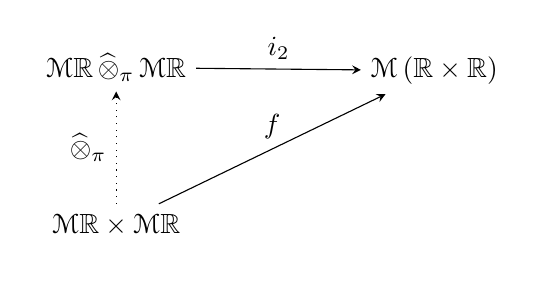
\begin{tikzpicture}
      \matrix (m) [matrix of math nodes, row sep=4em, column sep=6em, minimum width=2em]
      {
         \mathcal{M}\mathbb{R} \,   \widehat{\otimes}_{\pi} \,   \mathcal{M}\mathbb{R} &  \mathcal{M} \left( \mathbb{R} \times \mathbb{R} \right)  \\
        \mathcal{M}\mathbb{R} \times \mathcal{M}\mathbb{R}   \\
      };
      \path[dotted, -stealth]
      (m-2-1) edge node [left] {$\widehat{\otimes}_{\pi}$} (m-1-1);
      \path[-stealth]
        (m-1-1) edge node [above] {$i_2$} (m-1-2)
        (m-2-1) edge node [above] {$f$} (m-1-2)
        ;
    \end{tikzpicture}

    Where $i_2:  \mathcal{M}\mathbb{R} \,   \widehat{\otimes}_{\pi} \,   \mathcal{M}\mathbb{R} \to  \mathcal{M} \left( \mathbb{R} \times \mathbb{R} \right) $ is an isomorphism defined as $i_{2}( \mu  \widehat{\otimes}_{\pi} \nu ) = \mu \otimes \nu $ 
    and the function $f: \mathcal{M}\mathbb{R} \times \mathcal{M}\mathbb{R}  \to \mathcal{M} \left( \mathbb{R} \times \mathbb{R} \right) $ is defined as $f((\mu, \nu)) = \mu \otimes \nu $. 
    The product measure $\mu \otimes \nu$ is defined as $\mu \otimes \nu (A \times B)= \mu(A)\cdot\nu(B).$
      This is the measure produced by the Carath\'{e}odory's extension theorem \cite{aliprantisBanachLattices1999}.
       Given that $\norm{\mu \otimes \nu}= \norm{\mu} \cdot \norm{\nu}$,  and $\norm{(\mu, \nu)}= \max\{\norm{\mu}, \norm{\nu}\}$, for $\norm{\mu} \leq 1$ and $\norm{\nu} \leq 1$, it follows that $f$ is a short map.

    \end{comment}

    Since the diagram below commutes, and all the operations involved are short maps (considering $f$ as $\sem{\emph{delta}_r}$ or $\sem{\emph{u}_{r,s}}$), it follows that, if $d(\mu, \mu')=\epsilon$, then we may postulate \(\emph{JumpL}_\mu =_{\epsilon} \emph{JumpL}_{\mu'}\). A similar diagram can be constructed using \(jr_{*}\), allowing us to apply the same reasoning to the corresponding axioms.

    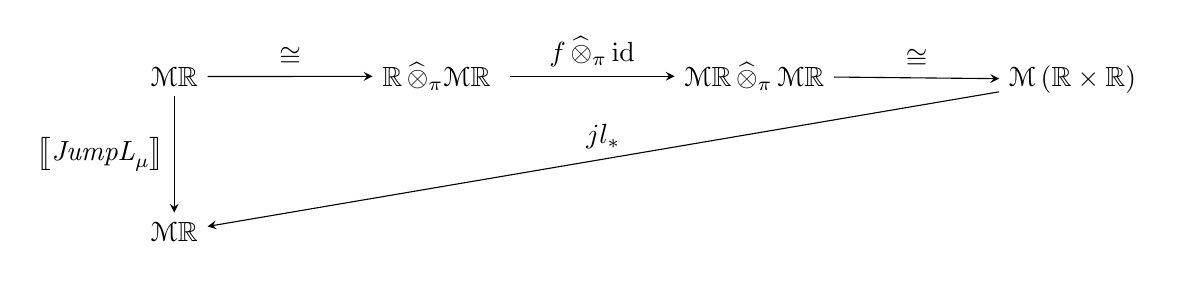
\begin{tikzpicture}
      \matrix (m) [matrix of math nodes, row sep=4em, column sep=6em, minimum width=2em]
      {
        \mathcal{M}\mathbb{R}  & \mathbb{R} \,   \widehat{\otimes}_{\pi} \mathcal{M}\mathbb{R} \,  \, & \mathcal{M}\mathbb{R} \, \widehat{\otimes}_{\pi} \,  \mathcal{M}\mathbb{R} &  \mathcal{M} \left( \mathbb{R} \times \mathbb{R} \right)  \\
        \mathcal{M}\mathbb{R}  \\
      };
      \path[-stealth]
        (m-1-1) edge node [left] {$\sem{\emph{JumpL}_\mu}$} (m-2-1)
        (m-1-1) edge node [above] {$\cong$} (m-1-2)
        (m-1-2) edge node [above] {$f\,  \widehat{\otimes}_{\pi} \,  \id $} (m-1-3)
        (m-1-3) edge node [above] {$\cong$} (m-1-4)
        (m-1-4) edge node [above] {$jl_{*}$} (m-2-1)
        ;
    \end{tikzpicture}

   We now present examples of \(\mu\) and \(\mu'\), and demonstrate how to compute the distance between them.
    First, consider $\mu=\delta_x$ and  $\mu'=\delta_y$. We calculate

    \begin{align*}
      \norm{\delta_x - \delta_y} = \sup \left\{ \sum_{i=1}^{n} |\delta_x - \delta_y (A_i)| \mid A_i \in \mathcal{B}(\mathbb{R}), A_i \cap A_j = \emptyset i,  \neq j, n \in \mathbb{N}  \right\} = 2
    \end{align*}
    Note that there are only two possibilities: either \(\delta_x\) and \(\delta_y\) belong to the same partition, or they belong to different ones. In the first case, we have
    \[
    \sum_{i=1}^{n} \left| \delta_x(A_i) - \delta_y(A_i) \right| = |1 - 1| = 0,
    \]
    while in the second case, we obtain
    \[
    \sum_{i=1}^{n} \left| \left( \delta_x(A_i) - \delta_y(A_i) \right) \right| = |1| + |-1| = 2.
    \]
    
    Next, take $\mu= \sum_{i=1}^{n} p_i \delta_{x_i}$ and  $\mu'= \sum_{i=1}^n q_i \delta_{x_i}$. We compute

    \begin{align*}
      \norm{\sum_i p_i \delta_{x_i} - \sum_i q_i \delta_{x_i}} &
      = \sup \left\{ \sum_{i=1}^{n} \left\lvert \left(\sum_i p_i \delta_{x_i} - \sum_i q_i \delta_{x_i} \right) (A_i) \right\rvert \,\Bigg| \, A_i \in \mathcal{B}(\mathbb{R}), A_i \cap A_j = \emptyset i,  \neq j, n \in \mathbb{N}  \right\} \\
      & = \sum_i |p_i-q_i|
    \end{align*}
    Here, we apply the same reasoning as in the previous example, while also using the inequality
\[
\left| \sum_{i=1}^{n} a_i \right| \leq \sum_{i=1}^{n} |a_i|, \quad \text{for all } n \in \mathbb{N}.
\]

Subsequently, let $\mu = U(a,b)$ and  $\mu'=U(c,d)$, such that the intervals $[a,b]$ and $[c,d]$ are disjoint ($[a, b] \cap [c, d] = \emptyset$). Then, the Radon-Nikodym derivatives (probability density functions) with respect to \( \nu = U(a, b) + U(c, d) \) are given by:

\[
\frac{dU(a, b)}{d\nu}(x) = u(a,b)(x) = 
\begin{cases} 
\frac{1}{b - a} & \text{if } x \in [a, b], \\ 
0 & \text{otherwise},
\end{cases}
\]
and similarly,
\[
\frac{dU(c, d)}{d\nu}(x) = u(c,d)(x) = 
\begin{cases} 
\frac{1}{d - c} & \text{if } x \in [c, d], \\ 
0 & \text{otherwise}.
\end{cases}
\]

Here, similarly to the first example, we calculate
\begin{align*}
  &\norm{U(a,b)-U(c,d)} = 2 \cdot \sup_{A \in \mathcal{B}(\mathbb{R})}  \left\{ \left\vert\int_A (u(a,b)(x)- u(c,d)(x)) \, d \nu(x) \right\vert \right\} \\
  & = 2 \cdot \sup_{A \in \mathcal{B}(\mathbb{R})}  \left\{ \left\vert\int_A (u(a,b)(x)) \, d \nu(x)  - \int_A (u(c,d)(x)) \,  d\nu(x) \right\vert \right\} = 2
\end{align*}

\begin{comment}
Here, we calculate
\begin{align*}
  \norm{U(a,b)-U(c,d)} = 2 \cdot \sup_{A \in \mathcal{B}(\mathbb{R})}  \left\{ \left\vert\int_A (u(a,b)(x)- u(c,d)(x)) \, dx \right\vert \right\} = 2 \cdot \sup_{A \in \mathcal{B}(\mathbb{R})}  \left\{ \left\vert\int_A (u(a,b)(x)- u(c,d)(x)) \, dx \right\vert \right\}
\end{align*}

In this case, we consider three scenarios: 
\begin{enumerate}
    \item The intervals are disjoint: \([a, b] \cap [c, d] = \emptyset\),
    \item One interval is fully contained in the other: for example, \([c, d] \subseteq [a, b]\) (or vice versa),
    \item The intervals intersect, but neither is fully contained in the other.
\end{enumerate}

In the first case, we have
\begin{align*}
  \int |u(a,b)(x)- u(c,d)(x)| \, dx  & = \int_a^b |u(a,b)(x)- u(c,d)(x)| \, dx + \int_c^d |u(a,b)(x)- u(c,d)(x)| \, dx \\
  & = \left\lvert \frac{b-a}{b-a}\right\rvert + \left\lvert- \frac{d-c}{d-c}\right\rvert = 2
\end{align*}

Regarding the second case, we compute
\begin{align*}
  \int |u(a,b)(x)- u(c,d)(x)| \, dx  & = \int_a^c |u(a,b)(x)- u(c,d)(x)| \, dx + \int_c^d |u(a,b)(x)- u(c,d)(x)| \, dx  \\
   & \hspace{10pt }+\int_d^b |u(a,b)(x)- u(c,d)(x)| \, dx \\
  & =  =  \frac{c-a}{b-a} + - (d-c) \left(\frac{1}{b-a} - \frac{1}{d-c}  \right)+  \frac{b-d}{b-a}
\end{align*}

At last, we calculate,
\begin{align*}
  \int |u(a,b)(x)- u(c,d)(x)| \, dx  & = \int_a^c |u(a,b)(x)- u(c,d)(x)| \, dx + \int_c^b |u(a,b)(x)- u(c,d)(x)| \, dx  \\
   & \hspace{10pt }+\int_b^d |u(a,b)(x)- u(c,d)(x)| \, dx \\
  & =  \frac{c-a}{b-a} +  (b-c) \left(\frac{1}{b-a} - \frac{1}{d-c}  \right)+  \frac{d-b}{b-a}
\end{align*}

\end{comment}

Finally, consider $\mu = \delta_{x_0} $  and $\mu' =  U(x_0 - \epsilon, x_0 + \epsilon) $. Let \(\nu = \delta_{x_0} + U(x_0 - \epsilon, x_0 + \epsilon) \). The Radon-Nikodym derivatives are:

\[
\frac{d\delta_{x_0}}{d\nu}(x) = f (x)
\begin{cases} 
1 & \text{if } x = x_0, \\
0 & \text{otherwise},
\end{cases}
\]

\[
\frac{dU(x_0 - \epsilon, x_0 + \epsilon)}{d\nu}(x) = u(x_0 - \epsilon, x_0 + \epsilon) = 
\begin{cases} 
\frac{1}{2\epsilon} & \text{if } x \in (x_0 - \epsilon, x_0 + \epsilon), \\
0 & \text{otherwise}.
\end{cases}
\]

We compute,
\begin{align*}
  \norm{\delta_{x_0}-U(x_0 - \epsilon, x_0 + \epsilon)} &= \sup_{A \in \mathcal{B}(\mathbb{R})} \left\{ \left\vert \int_A (f(x)- u(x_0 - \epsilon, x_0 + \epsilon) (x))\, d\nu(x) \right\vert \right\} \\
  &= \sup_{A \in \mathcal{B}(\mathbb{R})} \left\{ \left\vert \int_A f(x)\, d\nu(x) -  \int_A   u(x_0 - \epsilon, x_0 + \epsilon) (x) \, d\nu(x) \right\vert \right\} = 2
\end{align*}
    

\bibliographystyle{alpha} 
\bibliography{biblio}


\end{document}
